\documentclass[12pt]{article}
\usepackage{graphicx} % Required for inserting images
\usepackage[margin=1in]{geometry}
\usepackage{setspace}
\usepackage{natbib}
\usepackage{hyperref}
\usepackage{endfloat}
\usepackage[scale=1]{sourceserifpro}
\hypersetup{
    colorlinks=true,
    linkcolor=blue,
    filecolor=magenta,      
    urlcolor=blue,
    citecolor    = black
    }
\setcitestyle{authoryear}
\title{\LARGE King and Cochrane: 
The Technological Treadmill and Racial Inequity in US Agriculture}
\author{Jared Hutchins$^{1*}$ and Jacopo De Marinis$^{2}$ \\  \quad  \\ $^1$ University of Illinois Urbana-Champaign \\ $^2$ Ulster University\\  \quad  \\  \quad  \\ $^*$ Correspondence to be sent to:\\ Jared Hutchins, Ph.D. \\Email - jhtchns2@illinois.edu \\ \quad \\ Date of First Submission: November 1, 2023 \\ \quad \\ Date of Acceptance: May 5, 2025 \\ \quad \\
Editor: Alessandro Bonanno}
\date{}
\begin{document}

\maketitle
\quad \\
\textbf{Key Words:} structural change, Black farmers, agricultural policy, equity\\
\textbf{JEL Codes:} Q15, Q18, J15 \\
\quad \\
\textbf{Acknowledgements:} The authors would like to acknowledge and thank Bobby J. Smith II, Sarah Janzen, Joe Janzen, Hope Michelson, Marin Skidmore, Lawrence Lucas, Waymon Hinson, and Jonathan Coppess for providing feedback and comments during the writing of this manuscript.

\newpage

\begin{abstract}
\singlespacing
Between 1920 and 1969, the number of Black farmers in the United States decreased from 14\% of all operators to 4\%. 
Using Martin Luther King Jr.’s critique of agricultural policy and Willard Cochrane’s theory of the technological treadmill, we explore how racial discrimination was linked to policies that led to structural change in US agriculture. 
We discuss three areas of policy, land, education, and financial assistance, and how policy in these areas contributed to worsening conditions for Black farmers between 1920 and 1970.
We then discuss how these policy areas are framed in today's policy environment and offer some future directions for research.\\
\textbf{Key Words:} structural change, Black farmers, agricultural policy, equity\\
\textbf{JEL Codes:} Q15, Q18, J15
\end{abstract}
\newpage
\section*{Introduction}

\doublespacing

In 1920, Black farmers were 14\% of farm operators, higher representation than Black people had in the general population at around 10\%. 
However, in only 50 years, Black farmers decreased to being only 4\% of operators  \citep{francis_black_2022,reynolds_black_2002}.
Figure \ref{operators} shows that Black farming reached its peak in 1920 but declined sharply between 1920 and 1970.
Today, Black farmers represent less than 2\% of operators \citep{USDA_black_farmers}.
Some policymakers have pointed to federal policy as the reason for this decline. 
Senator Cory Booker, a Senate sponsor for the Justice for Black Farmers Act, alleged a \textit{``direct connection between discriminatory USDA policies and the enormous land loss we have seen among Black farmers''} \citep{booker_booker_2023}. 

Yet, the structural changes happening in agriculture from 1920 to 1970 could provide an alternative explanation.
In those 50 years, productivity growth from technological change was a significant driver of output growth and the number of farms dropped precipitously as the population began transitioning away from farming and rural areas altogether \citep{dimitri_20th_2005,mundlak_economic_2005}.
The structural change theory pioneered by Willard Cochrane, called the technological treadmill, emphasizes that productivity growth can erode profits in agriculture and drive farmers out of the sector when they do not adopt technology quickly enough \citep{cochrane_farm_1958,levins_treadmill_1996}.
The decline in Black farmers between 1920 and 1970 thus could be understood as the natural consequence of structural change predicted by the technological treadmill and not a result of discrimination.



\begin{figure}[ht!]
\caption{Total Number and Percentage of Black Operators: 1900-1997}
\label{operators}
\centering
    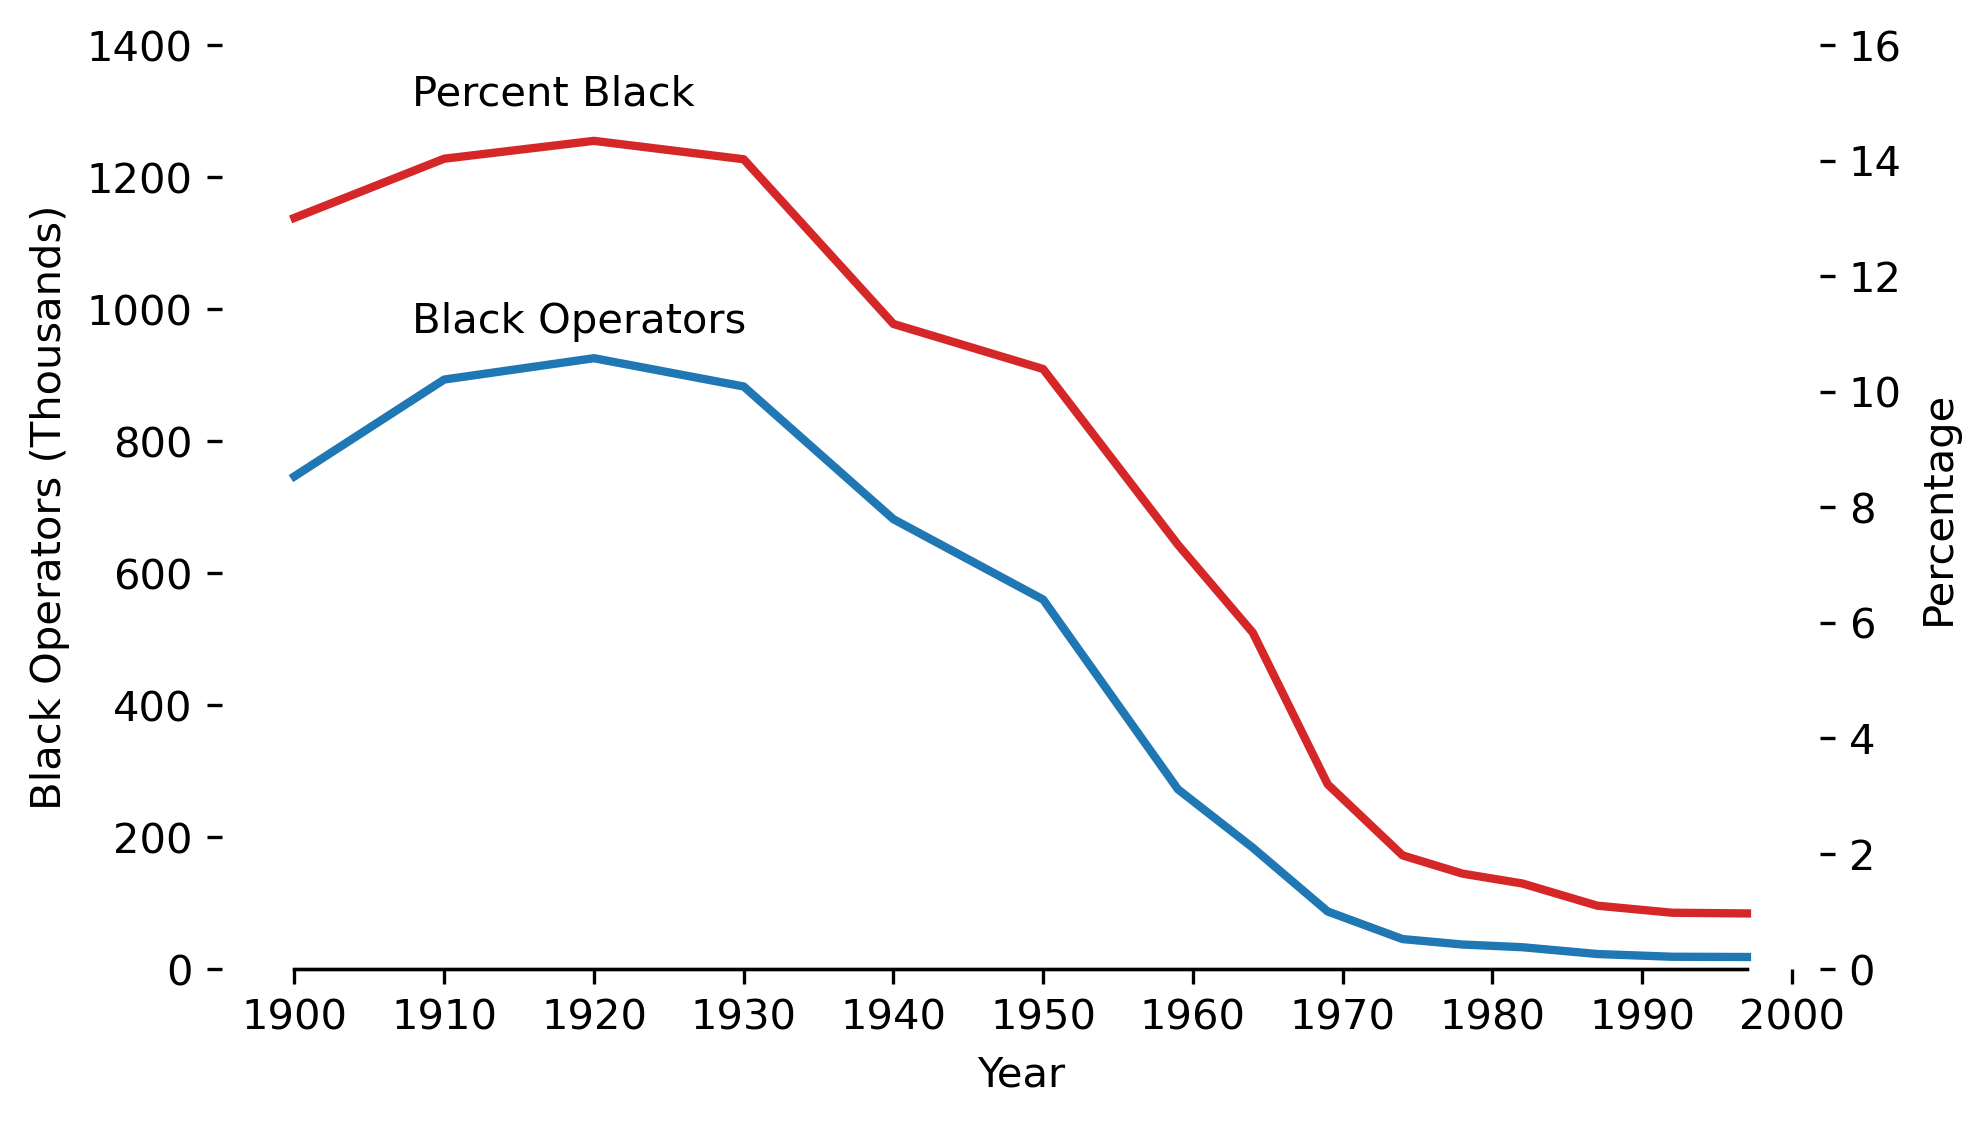
\includegraphics[width=.9\textwidth]{figs/Figure1.png}
    
Source: US Agricultural Census, reported in \citet{reynolds_black_2002}, Appendix Table 3

\end{figure}


In this paper, we explore the complicated relationship between racial discrimination and US agricultural policy during an era of major structural change: 1920 to 1970. 
Using historical accounts and data sources, we examine how policy could have mediated the impacts of the technological treadmill to fall harder on Black farmers compared to other farmers in some key policy areas.
Marching with the Poor People’s Campaign in 1968, Dr. Martin Luther King highlighted these important policy areas in a speech: 


\begin{quote}
“At the very same time that America refused to give the Negro any land, through an act of Congress, our government was \textbf{giving away millions of acres of land} in the West and the Midwest… 
But not only did they give the land, \textbf{they built Land Grant Colleges} with government money to teach them how to farm. 
Not only that, they \textbf{provided county agents} to further their expertise in farming. 
Not only that, they provided \textbf{low interest rates} in order that they could mechanize their farms. 
Not only that, today many of these people are receiving \textbf{millions of dollars in federal subsidies not to farm} and they are the very people telling the Black man that he ought to lift himself by his own bootstraps.” 
\begin{center}
- Dr. Martin Luther King Jr., quoted in \citet{dyson_i_2000}, pg. 12 (emphasis added) \end{center}
\end{quote}

In this quote, King highlights three critical areas of agricultural policy: land, education, and financial assistance. 
King challenges an implicit assumption that Cochrane largely took as granted: that the agricultural sector was a meritocracy where a farmer could ``lift himself by his own bootstraps.''
Because Cochrane's treadmill theory primarily sees technology adoption as determined by how ``industrious'' a farmer is, Cochrane did not consider how US government policy determines who the technology treadmill affects. 
For over a century, farmers received significant assistance from the federal government in the form of land transfers, extension programs, and government subsidies and loans.
If the government discriminated on race in these key policy areas, the policies would be inadvertently picking the winners and losers of the technological treadmill along racial lines.

Focusing on 1920 to 1970, this paper explores historical accounts and data series to document instances where agricultural policy concerning land, education, and financial assistance was skewed to the benefit of white farmers to the detriment of Black farmers. 
In many of the debates surrounding influential policies such as the Morrill Act and the Smith-Lever Act, we find instances in which policy-makers and USDA officials advocated against Black farmers receiving resources equal to white farmers, sometimes citing a belief that Black farmers were in some way inferior and should not be treated the same \citep{harris_extension_2008,rose_race_2022,davis_negro_1933,poe_south-wide_1913}.
Case studies throughout this period also find instances of white farmers organizing to prevent Black farmers from buying land or being represented on county committees in charge of granting loans and subsidies \citep{daniel_dispossession_2013,irons_reconstituting_2010,black_economic_research_center_center_only_1973}.
Other data from Censuses, statistical bulletins, and reports document patterns of higher rates of tenancy among Black farmers in 1920, less funding for Black farmer education and extension, and unequal treatment by county committees and loan programs \citep{wilkerson_agricultural_1942,us_commission_on_civil_rights_equal_1965,reynolds_black_2002}.
By being denied these resources, Black farmers could have been less likely to weather Cochrane’s treadmill the way that white farmers did in the early 20th century. 

Our work primarily contributes to ongoing research that explores how past economic policy has exacerbated racial inequality in agriculture. 
Recent work in agricultural economics has surveyed the historical context of land policy \citep{muhammad_african_2024,darity_jr_reconsidering_2023,francis_black_2022} and agricultural education policy \citep{grant_overview_2024,wilson_distribution_2024} to explain how past inequities have contributed to racial inequality today.
Other work has focused on documenting the disparities that persist today in government payments \citep{giri_analysis_2022,hendricks_explaining_2023,yu_understanding_2024} and credit markets \citep{mishra_racial_2024,vekemans_loan_2024,mcdonald_role_2022,ahrendsen_beginning_2022}. 

The primary contribution of this paper is applying this critical lens to analyzing the policies that spurred structural change and mechanization in US agriculture. 
Our work contributes to this field of agricultural economics by first re-examining implicit assumptions of Cochrane's treadmill and examining historical evidence of racial discrimination in areas that the theory predicts to be relevant to the effects of the treadmill. 
Reframing our understanding of structural change in US agriculture is essential for agricultural economics to better consider issues of justice and inequity in both teaching and researching agricultural policy in the US \citep{wilson_call_2023,darity_jr_reconsidering_2023}. 

We first explain the technological treadmill theory and how it helps us understand the experience of Black farmers in structural change. We then use King’s three main categories of policy – land, education, and financial assistance – to give a brief, non-exhaustive summary of qualitative and quantitative evidence that the benefits of policies were skewed towards white farmers at the detriment of Black farmers. While racial discrimination persisted after 1970, we specifically focus on the factors that led to the significant drop in Black farmer participation from 1920 through the 1960s. We conclude by reviewing where future research might build on our analysis and better understand racial discrimination and structural change in US agriculture.


\section*{Cochrane’s Treadmill Theory and Discrimination}
Cochrane’s treadmill theory aims to predict how exogenous technological change in a competitive agricultural market impacts farm profitability.
By racing to adopt technology that expands output, farmers inadvertently eat away the profits they earned from adoption by pushing down the output price until farmers are either back where they started or can no longer afford to keep farming \citep{cochrane_farm_1958}.
Over time, the increased competitiveness of farming can produce the outcome we see today: a more productive farming sector with a far smaller number of farms.
Compared to other structural change theories, such as Sir Arthur Lewis' two-sector model, Cochrane puts special emphasis on productivity-enhancing technology as a driving force of this change.

Cochrane's focus on technological innovation reflects the fact that, by the time the technological treadmill theory was published in 1958, improvements in seed genetics, capital, and chemical fertilizers had been pushing up output for decades \citep{mundlak_economic_2005}.
Cochrane predicted that the benefits of productivity-enhancing technology for farmers would depend on their speed of adoption.
He breaks farmers roughly into three groups: early-adopters, average farmers, and laggards.
``Early-adopters'' are farmers who adopt early enough to enjoy the profits from the technology before output prices decrease.
The next round of adopters, the ``average farmers,'' may adopt just in time to see themselves break even with the new technology. 
The latest adopters, the ``laggards,'' would see their profits eaten away before they might even be able to adopt the new technology and would be put out of business.
In the spirit of Schumpeter’s creative destruction, the remaining farmers can divide up the resources of the laggards and expand their operations, leading to yet another increase in output \citep{cochrane_farm_1958}. 

In this form of the theory, the primary impact on farmers is through a declining output price.
However, when Cochrane formulated it in 1958, the USDA was already busy insulating US farmers against output price fluctuations with non-recourse loans and commodity purchases. 
In 1965, Cochrane amended the theory to explain how increased government supports would not save farmers from the treadmill.
As the government continued to subsidize farming, these supports would be capitalized into land prices and increase rents. 
While farmers who own land would reap the benefits of the land price increases, renters would see their profits eaten away by the rent increases \citep{cochrane_city_1965}. 
Between 1959 and 1969, land prices increased about 34\%, leading economists like D. Gale Johnson and Luther Tweeten to give additional scrutiny to the impact of farm programs on land prices \citep{johnson_farm_1973,tweeten_foundations_1970}. 

\citet{cochrane_development_1993} revised the theory once again to explain how land ownership might impact the outcomes of the technological treadmill.
If farmers are all renters, then the theory is unchanged: farmers are squeezed by the rising costs of their land instead of a decrease in output price. 
If a farmer owns their land, however, they reap the benefits of their land values going up. 
\citet{levins_treadmill_1996} calls this the ``land market treadmill'' and predicted that this process would not only lead to a speedy exit for renting farmers but also raise the barriers to entry for new farmers.

The treadmill theory in all its forms is built on the idea that some farmers adopt technology faster than others.
What, in Cochrane's mind, made a farmer an ``early-adopter''?
While \citet{cochrane_city_1965} recognized the Land Grant University (henceforth LGU) system as one way farmers discovered new technology, he often attributed early adoption to skill, characterizing early adopters with words like “industriousness” and “astute” and characterizing laggards as \textit{``the lazy fellow who would rather go fishing''}\citep{cochrane_farm_1958,cochrane_city_1965}. 

Today, the economics field understands technology adoption decisions to be a function of more than just innate, individual skill.
Training and education programs play a critical role in stimulating uptake of new technologies \citep{pan_agricultural_2018,takahashi_technology_2020}.
Recent work shows that extension programs, in particular, can be an essential source of information for farmers to learn about new technologies and how to apply them \citep{deutschmann_can_2019,kondylis_seeing_2017}.
Moreover, even well-trained farmers may not adopt technology because they lack access to credit \citep{karlan_agricultural_2014,regassa_access_2023}.
Studies also show that insurance programs that reduce price or yield risk for farmers can also have positive impacts on technology uptake \citep{karlan_crop_2011,arouna_contract_2021,carter_where_2016}.

All of these factors impacting technology adoption are greatly influenced by government policies that provide education and financial assistance for farmers.
Thus, federal policy in the US played a crucial role in determining the impacts of the technological treadmill in the 20th century by providing farmers with land, training, and access to credit, all factors that determine success on the treadmill.
Yet, when there is discrimination in federal policy, this opens up the possibility that discrimination will skew the benefits of government policy towards one group and away from another.
Thus, discrimination can be a factor in selecting the early-adopters and laggards of the treadmill and can prevent the most ``industrious'' farmers from rising to the top.
A systematic preference for a certain group of farmers in government policy is the sort of possibility that is absent from any of Cochrane's theories.
However, it is an essential insight for understanding which farmers survived the technological treadmill between 1920 and 1970.




\section*{Land Policy}
Land ownership is an important factor for surviving Cochrane's treadmill, as it translates rising land prices into a benefit instead of a cost.
The US government strongly influenced who felt the impact of the treadmill by granting land and giving loans to tenants to buy land.
Beginning in the 19th century, the western territories were parceled out to settlers in a series of homestead acts. 
The largest of these land transfers was the Homestead Act of 1862, signed by President Lincoln in the middle of the Civil War. 
Over 76 years, the 1862 Act distributed 246 million acres of land (close to the size of California and Texas combined) to 3 million individuals, making it one of the largest asset transfer programs in US history \citep{williams_shanks_homestead_2000}. 

Few Black Americans benefited from the Homestead Act. 
Before the abolition of slavery, the Dred Scott decision of 1857 established that Black Americans were not considered citizens and could not apply for Homestead Act allotments \citep{muhammad_african_2024}. 
Even after the abolition of slavery in 1865, the Black Codes in Southern states drastically restricted Black social mobility, significantly hampering their ability to migrate and take advantage of homestead allotments \citep{meredith_black_1940}.  
Moreover, even if they had the resources to migrate, many freed slaves after 1865 also lacked the resources and capital to transform homesteaded land into farmland \citep{edwards_african_2019,muhammad_african_2024}. 

After the Civil War, there were efforts to redistribute plantation land in the South to newly freed slaves. 
General William T. Sherman issued Field Order No. 15 in January of 1865 which ordered “40 acres and a mule” for former slaves by appropriating land along the coast in South Carolina and Georgia \citep{special_field_orders_no_15_order_1865}. 
More formally, Congress passed the Southern Homestead Act (henceforth SHA) of 1866, a homestead program that aimed to parcel out 80- and 160-acre allotments from Confederate territory to freed slaves and northern whites \citep{williams_shanks_homestead_2000}. 
However, Lincoln's successor Andrew Johnson and House Democrats undermined the efficacy of the SHA in benefiting freed slaves by removing the provision that barred ex-confederates from applying \citep{williams_shanks_homestead_2000}.
While Black homesteaders made more improvements to their land than white homesteaders, only 23\% of SHA claimants were Black and only 6\% of the originally promised land was distributed before the SHA was repealed in 1876 \citep{canaday_race_2015,lanza_agrarianism_1999}.

Entering the 20th century, helping tenant farmers transition into land ownership became a common focus of policy debates.
Despite the fact that a large portion of Black farmers were tenants, white tenants appeared most often as the focus of policy.
One example of a passionate defender of white tenants but a critic of Black farmers was Clarence Poe, the editor of one of the most widely read agricultural publications of the time, The Progressive Farmer \citep{cote_clarence_1979}. 
Poe was a passionate defender of poor white tenants who, at the same time, argued that Black farmers made no contribution to society \citep{poe_what_1915}. Poe, as a proponent of segregation, also argued that white property owners should be allowed to prohibit Black families from buying property in their community to stop the crowding out of white families \citep{poe_south-wide_1913}. 

Poe’s influence on policy debates is evidenced by the fact that his letters and op-eds appeared several times in the Congressional Record in the 1930s \citep{78_cong_rec_5476_congressional_1934,79_cong_rec_685_congressional_1935}. 
Notably, Poe was called to testify to the Senate Agriculture Committee on the Bankhead-Jones Act, a loan program to help tenants become land owners, and argued passionately for the welfare of poor white tenants who he felt were being treated as inferiors \citep{75th_cong_355_farm_1937}. 
The focus on the plight of the white tenants appeared to bear out in the implementation of the program, as Black farmers, by 1949, made up of 50\% of southern tenants but only 23\% of the loan recipients \citep{banfield_ten_1949}. 

The vocal support for segregation in some Southern states also had implications for Black farmers looking to buy land.
In a 1913 op-ed, Poe wrote that \textit{``few home-owners would dare sell a home to a Negro right on a prominent white street. The same sort of sentiment can accomplish much in the country''} \citep[pg. 845]{poe_south-wide_1913}.
\citet{brown_successful_1977} presents case studies from the 1960s showing that this kind of ``sentiment'' was often a significant barrier to Black farmland ownership in the South. In a 1973 report by the Black Economic Research Center, field agents even detailed incidents in the Deep South where white farmers conspired with local bankers to push Black farmers into debt and poverty to have leverage to buy their land \citep{black_economic_research_center_center_only_1973}. Racialized violence against Black communities in the South, where most Black farmers resided, also encouraged Black families to abandon their landholdings and follow other families in the Great Migration \citep{daniel_dispossession_2013,wilkerson_long-lasting_2016}.
Having left their land, much of the holdings were then left vulnerable to developers who could force sales on land owned fractionally by taking advantage of heirs’ property laws \citep{mitchell_reconstruction_2000}.

\begin{table}
\caption{Land in Farms and Number of Operators by Type of Ownership and
Operators’ Race: 1920 and 1959}
\label{operator_acrage}
\centering
\footnotesize
\begin{tabular}{llrrrr}
\hline
        &           &     &     &   \\
 &  &    1920 &     1959 & \textit{Change} &  \textit{\% Change} \\
[.5em]
\hline 

\multicolumn{6}{c}{\textit{Acres (Millions)}} \\
[.5em]
Owner & Total & 4,612.50 & 3,464.03 & -1,148.47 & -24.90 \\
 & White & 4,472.45 & 3,398.18 & -1,074.27 & -24.02 \\
 & Non-white & 140.05 & 65.85 & -74.20 & -52.98 \\
 & \% Non-white & 3.04 & 1.90 & -1.14 &  \\
 [1em]
Part Owner & Total & 1,755.25 & 5,029.32 & 3,274.07 & 186.53 \\
 & White & 1,728.26 & 4,975.99 & 3,247.73 & 187.92 \\
 & Non-white & 26.99 & 53.33 & 26.34 & 97.59 \\
 & \% Non-white & 1.54 & 1.06 & -0.48 & \\
 [1em]
Tenant & Total & 2,649.80 & 1,631.84 & -1,017.96 & -38.42 \\
 & White & 2,372.15 & 1,576.41 & -795.74 & -33.55 \\
 & Non-white & 277.65 & 55.43 & -222.22 & -80.04 \\
 & \% Non-white & 10.48 & 3.40 & -7.08 &  \\
 [1em]
All & Total & 9,017.55 & 1,0125.19 & 1,107.64 & 12.28 \\
 & White & 8,572.86 & 9,950.58 & 1,377.72 & 16.07 \\
 & Non-white & 444.69 & 174.61 & -270.08 & -60.73 \\
 & \% Non-white & 4.93 & 1.72 & -3.21 &  \\
 [.5em]
\hline 


\multicolumn{6}{c}{\textit{Operators (Thousands)}} \\
[.5em]
Owner & Total & 3,367.81 & 2,114.20 & -1,253.61 & -37.22 \\
 & White & 3,174.68 & 2,016.81 & -1,157.87 & -36.47 \\
 & Non-white & 193.13 & 97.39 & -95.74 & -49.57 \\
 & \% Non-white & 5.73 & 4.61 & -1.13 &  \\
[1em]
Part Owner & Total & 558.71 & 833.15 & 274.44 & 49.12 \\
 & White & 517.82 & 792.42 & 274.60 & 53.03 \\
 & Non-white & 40.89 & 40.73 & -0.16 & -0.39 \\
 & \% Non-white & 7.32 & 4.89 & -2.43 &  \\
[1em]
Tenant & Total & 2,458.54 & 733.44 & -1,725.10 & -70.17 \\
 & White & 1,740.53 & 592.42 & -1,148.11 & -65.96 \\
 & Non-white & 718.01 & 141.02 & -576.99 & -80.36 \\
 & \% Non-white & 29.20 & 19.23 & -9.98 & \\
[1em]
All & Total & 6,385.06 & 3,680.79 & -2,704.27 & -42.35 \\
 & White & 5,433.03 & 3,401.65 & -2,031.38 & -37.39 \\
 & Non-white & 952.03 & 279.14 & -672.89 & -70.68 \\
 & \% Non-white & 14.91 & 7.58 & -7.33 &  \\
\hline \hline
\end{tabular}


Source: US Agricultural Census 1959, Volume 2, Chapter X, Tables 4 and 6
\end{table}

Using the Agricultural Census, we can see roughly how Black farmland ownership looked in 1920 and how it evolved through 1959 in this policy environment.
Table \ref{operators} shows the change in operators and acreage by type (owner, part-owner, and tenant) and by race (white and non-white) as reported in the 1959 Agricultural Census.\footnote{The 1959 Agricultural Census includes the following categories in its definition of ``tenant'': cash tenant, crop share tenant, cash and share tenant, sharecropper, and ``other.'' The Census defines ``part-owner'' as farmers that ``operate land they own and also land rented from others.'' Another tenure category that the Census reports on but we do not use in the analysis is ``manager.'' For this period, the Agricultural Census gives no further breakdown by race other than "white" and "non-white." The term ``non-white,'' while not specifically referring to Black farmers, is a suitable proxy since, according to the 1959 Agricultural Census, nearly 90\% of non-white farmers were Black. }
In general, we see a pattern of consolidation from 1920 to 1959 where total acreage increased 12\% and the number of operators decreased 42\%.
Yet, there are clear disparities across race: non-white farmer acreage dropped by 60\% versus white farmer acreage which increased 16\%.
Breaking down these patterns across race, some relevant observations are that i) non-white farmers were predominantly tenants in 1920, ii) non-white farmers were more likely to have small farms in 1920, and iii) non-white operators and acreage saw larger declines in this period than their white counterparts in the same ownership category. 

In 1920, Black farmers were likely overrepresented in agriculture since non-white people were 14\% of farming operators compared to 9.8\% of the country's population being Black \citep{Census1921}.
However, non-white farmers were also overrepresented in tenancy: non-white farmers made up only 5\% of land owners but 29\% of tenants. 
Similar racial disparities are visible in the growth of part owners. 
Between 1920 and 1959, the number of acres operated by white part-owners increased by 180\% but only 90\% for non-white part-owners. 
The number of white part-owners grew by 50\% while that of non-white part-owners changed very little. 
Being predominantly tenants explains part of the drop in non-white acreage since the number of tenant farmers decreased 70\% between 1920 and 1959 versus 37\% for owners, and the number of acres operated by tenants decreased by about 40\% versus 25\% for owners.

Another disparity across race may have been the average size of farms in 1920. 
While reliable data on farm size across race is unavailable in these years, the ratio of total acres to total operators is a proxy to show differences across race in these aggregate data. 
The ratio for non-white farmers was 46 acres in 1920 versus 157 acres for white farmers. 
By 1959, this ratio had grown 85\% for white farmers but only 33\% for non-white farmers. 
The 33\% growth for non-white farmers was entirely from growth in the ratio of acres to operators for part-owners, as this ratio for non-white tenants grew only 1.65\% and for non-white owners shrank 6.5\%. 
In contrast, this ratio grew 95\% for white tenants and about 20\% for white owners. 
In addition to being predominantly tenants, the initial disparities in farm size in 1920 may have disadvantaged non-white farmers in expanding their landholdings and garnering financial support to mechanize in this period.

Still, even within the same tenure category, non-white farms lost more operators and acreage than white farms.
From 1920 to 1959, the number of white tenants dropped by 65\% compared to 80\% for non-white tenants. 
The decline in land operated by tenants was even less equitable across race: tenant-operated land dropped by 33\% for white operators and by a much larger 80\% for non-white operators. 
The number of full owners dropped by similar amounts for white (36.47\%) and non-white (49.57\%) operators, though the percentage drop in non-white owned acreage was twice that of white-owned acreage (53\% versus 24\%). \footnote{This pattern holds even when considering farmers outside the South, where fewer Black farmers were concentrated in crops that would see rapid mechanization during this period. For trends broken down by South and non-South, see Online Appendix A.}
Thus, even non-white farms with the same type of ownership as white farms appear to have lost disproportionately more land in this period. 

While quantitative studies of Black land loss between 1920 and 1960 were rare, more recent studies have explored the implications of Black farmers receiving less land before 1920.
\citet{darity_jr_reconsidering_2023} estimates that the promised 40-acre tract of land would roughly be worth between \$175-480 thousand for a family today. 
\citet{miller_righteous_2020} examines the outcomes of freed slaves in the Cherokee territories where they were given land as compared to similar Southern Black households. 
They find that Black households who were granted land had more productive farms and had higher levels of education even decades later.
As for total Black land loss, \citet{francis_black_2022} estimates that Black households lost \$326 billion worth of land, or \$4 billion a year, between 1920 and 1997. 


\section*{Education Policy}
The Morrill Act of 1862 formed the LGU system, placing a university aimed at research and technical training in every state \citep{sorber_land-grant_2018}. 
The LGU system not only played an important part of increasing on-farm productivity and innovation through its research mission \citep{andrews_local_2021,kantor_research_2019} but also in spurring technology adoption and mechanization among farmers through its outreach mission.
As Cochrane's treadmill places central importance on technological progress, the LGU system plays a critical role in Cochrane's theory of structural change since it both creates and distributes the benefits of technological progress in agriculture.

To understand how racial discrimination may have mediated the impacts of the treadmill, it is important to understand how attitudes towards Black farmers impacted the formation and development of both the initial LGUs created in 1862 and those created in 1890 to serve Black farmers, called the 1890 LGUs.\footnote{For a more comprehensive treatment of the story of the 1890 LGUs, we refer readers to research on the history of the system via \citet{sorber_land-grant_2018}, \citet{rose_race_2022}, and \citet{sharpe_all_2004} and recent work on the inequities in the LGU system today via \citet{grant_overview_2024}, \citet{wilson_distribution_2024} and \citet{adams_how_2022}.} 
After the passage of the Morrill Act of 1862, lawmakers drafted the Morrill Act of 1890 to shore up more financial support for the LGU system. 
Since Black students were not allowed to attend LGUs in states that enforced segregation, Republican politicians and activists leveraged this renewed political interest in the LGU system to advocate for racial equity in education. 
This led to the passage of a second Morrill Act in 1890 which both funded the LGUs and barred states from receiving federal dollars if their LGU discriminated based on race \citep{rose_race_2022}.
However, states with segregation could still receive federal money if they set up another equivalent LGU specifically for non-white students. 
The universities created to comply with this restriction are referred to as “1890 Land Grant Universities” while those created with the original act are “1862 Land Grant Universities.” 

The Morrill Act of 1890 explicitly mandated\textit{ “a just and equitable division of the fund to be received under this act between one college for white students and one institution for colored students”} \citep[pg. 314]{davis_negro_1933}.
However, the policy apparatus made it difficult for 1890 LGUs to receive a proportionate amount of funds.
Since there was no dedicated funding source for 1890 LGUs, dispersing federal dollars to 1890 LGUs was left up to the discretion of the state legislature \citep{davis_negro_1933,harris_extension_2008}. 
Federal funds to LGUs had to be matched, usually by funds from the state legislature, and state legislatures often did not match 1890 funds or intentionally withheld funds from 1890 LGUs. 
\citet{davis_negro_1933} estimates that in 1930, no 1890 LGU received more than half of the funds that were expressly set aside for them from the Morrill Act of 1890. 

The LGU extension programs were created by Smith-Lever Act of 1914.
During the debates around Smith-Lever, attempts were made to ensure that Smith-Lever funds were shared equally between 1890 and 1862 LGUs. 
The Jones Amendment proposed that a direct appropriation be made for 1890 LGUs in the Smith-Lever funds rather than leaving it to the discretion of the state legislature. 

However, the Congressional Record of debates in the Senate surrounding the Jones Amendment in 1914 reveals that some senators relied on white supremacist arguments to keep this authority with the state legislature.
With regards to the disbursement of funds, Senator Vardaman argued that “You can not with any sort of prudence or any hope for good results leave the disbursement of this money, or any part thereof, in any other hands except those of the white people” \citep{51_cong_rec_2651-2_congressional_1914}.
One of Smith-Lever’s sponsors, Senator Hoke Smith, agreed and referred to Black farmers as “a backward, uninitiative, unintelligent, incapable black race” in the Congressional Records \citep{51_cong_rec_2651-2_congressional_1914}. 
Southern senators argued that, while Black farmers should still be counted in the rural population used to determine the amount of funds, the authority to disperse those funds should be held by the state legislature and the 1862 LGUs \citep{harris_extension_2008}. 
In the end, these arguments won out and the Jones Amendment was defeated.

\citet{baker_negro_1939} reported that extension directors avoided funding the Black extension program, called the Negro Extension Service, because they feared having to report that funding to their state legislators. 
Yet, in 1941, Secretary of Agriculture Claude Wickard claimed that the Negro Extension Service did not need separate Smith-Lever funds because white extension agents were already sufficiently serving Black farmers.
Black extension agents were only needed to supplement the extension work of white agents. 
He also claimed that, while only 14\% of funding was devoted to the Negro Extension Service, this was more than equitable because Black farmers only operated 9.47\% of the South’s farmland \citep{wickard_extension_1941}.

The Conference of the Presidents of Negro Land Grant Colleges responded to these claims by presenting evidence that Black farmers and extension agents were not being treated equitably by white extension agents.
They also challenged the idea that fund allocation should be based on acreage, as the funding formulas were based on rural population and not acreage.
Using data on extension funding, they calculated that state legislatures should have allocated \$1.9 million more in 1940 to be proportional to the Black, rural population \citep{wilkerson_agricultural_1942}.


In addition to a lack of funding, extension programs for Black farmers were also hampered by what white extension agents appeared to believe about the capabilities of Black farmers.
When the US Commission on Civil Rights interviewed extension agents in 1965, many agents and directors argued that Black farmers did not need the same education as white farmers.
One state program stated that training for Black agents and farmers should specifically be directed \textit{``within the context of the role expectations held for them by society''} \citep[pg. 33]{us_commission_on_civil_rights_equal_1965}. 
In interviews with white extension agents, the Commission on Civil Rights also found that Black farmers were discouraged from growing corn or keeping livestock \citep{us_commission_on_civil_rights_equal_1965}.
One extension agent even said that he would not train Black farmers in dairying because he did not believe that Black farmers would work seven days a week \citep[pg. 37]{us_commission_on_civil_rights_equal_1965}. 

Consistent with these attitudes, the Commission found some clear cases where Black farmers and extension agents received less training than their white counterparts.
In Georgia, white county agents received training in thirteen subjects while Black agents received only two \citep[pg. 31]{us_commission_on_civil_rights_equal_1965}. 
In Virginia, white agents received a two-week training course just on tobacco and six different meetings on peanut disease. 
In contrast, Black agents were only given a two-day meeting covering tobacco, peanuts, soybeans, weeds, and fertilizer \citep[pg. 32]{us_commission_on_civil_rights_equal_1965}.
The Commission even found that, due to a lack of funding, many Black extension offices lacked electricity, running water, and basic office supplies \citep[pg. 29]{us_commission_on_civil_rights_equal_1965}.

\begin{figure}
\caption{Percent of Total LGU Funding to 1890 LGUs versus Black Population: 1900 and 1931}
\label{1890LGUfunds}
\centering
    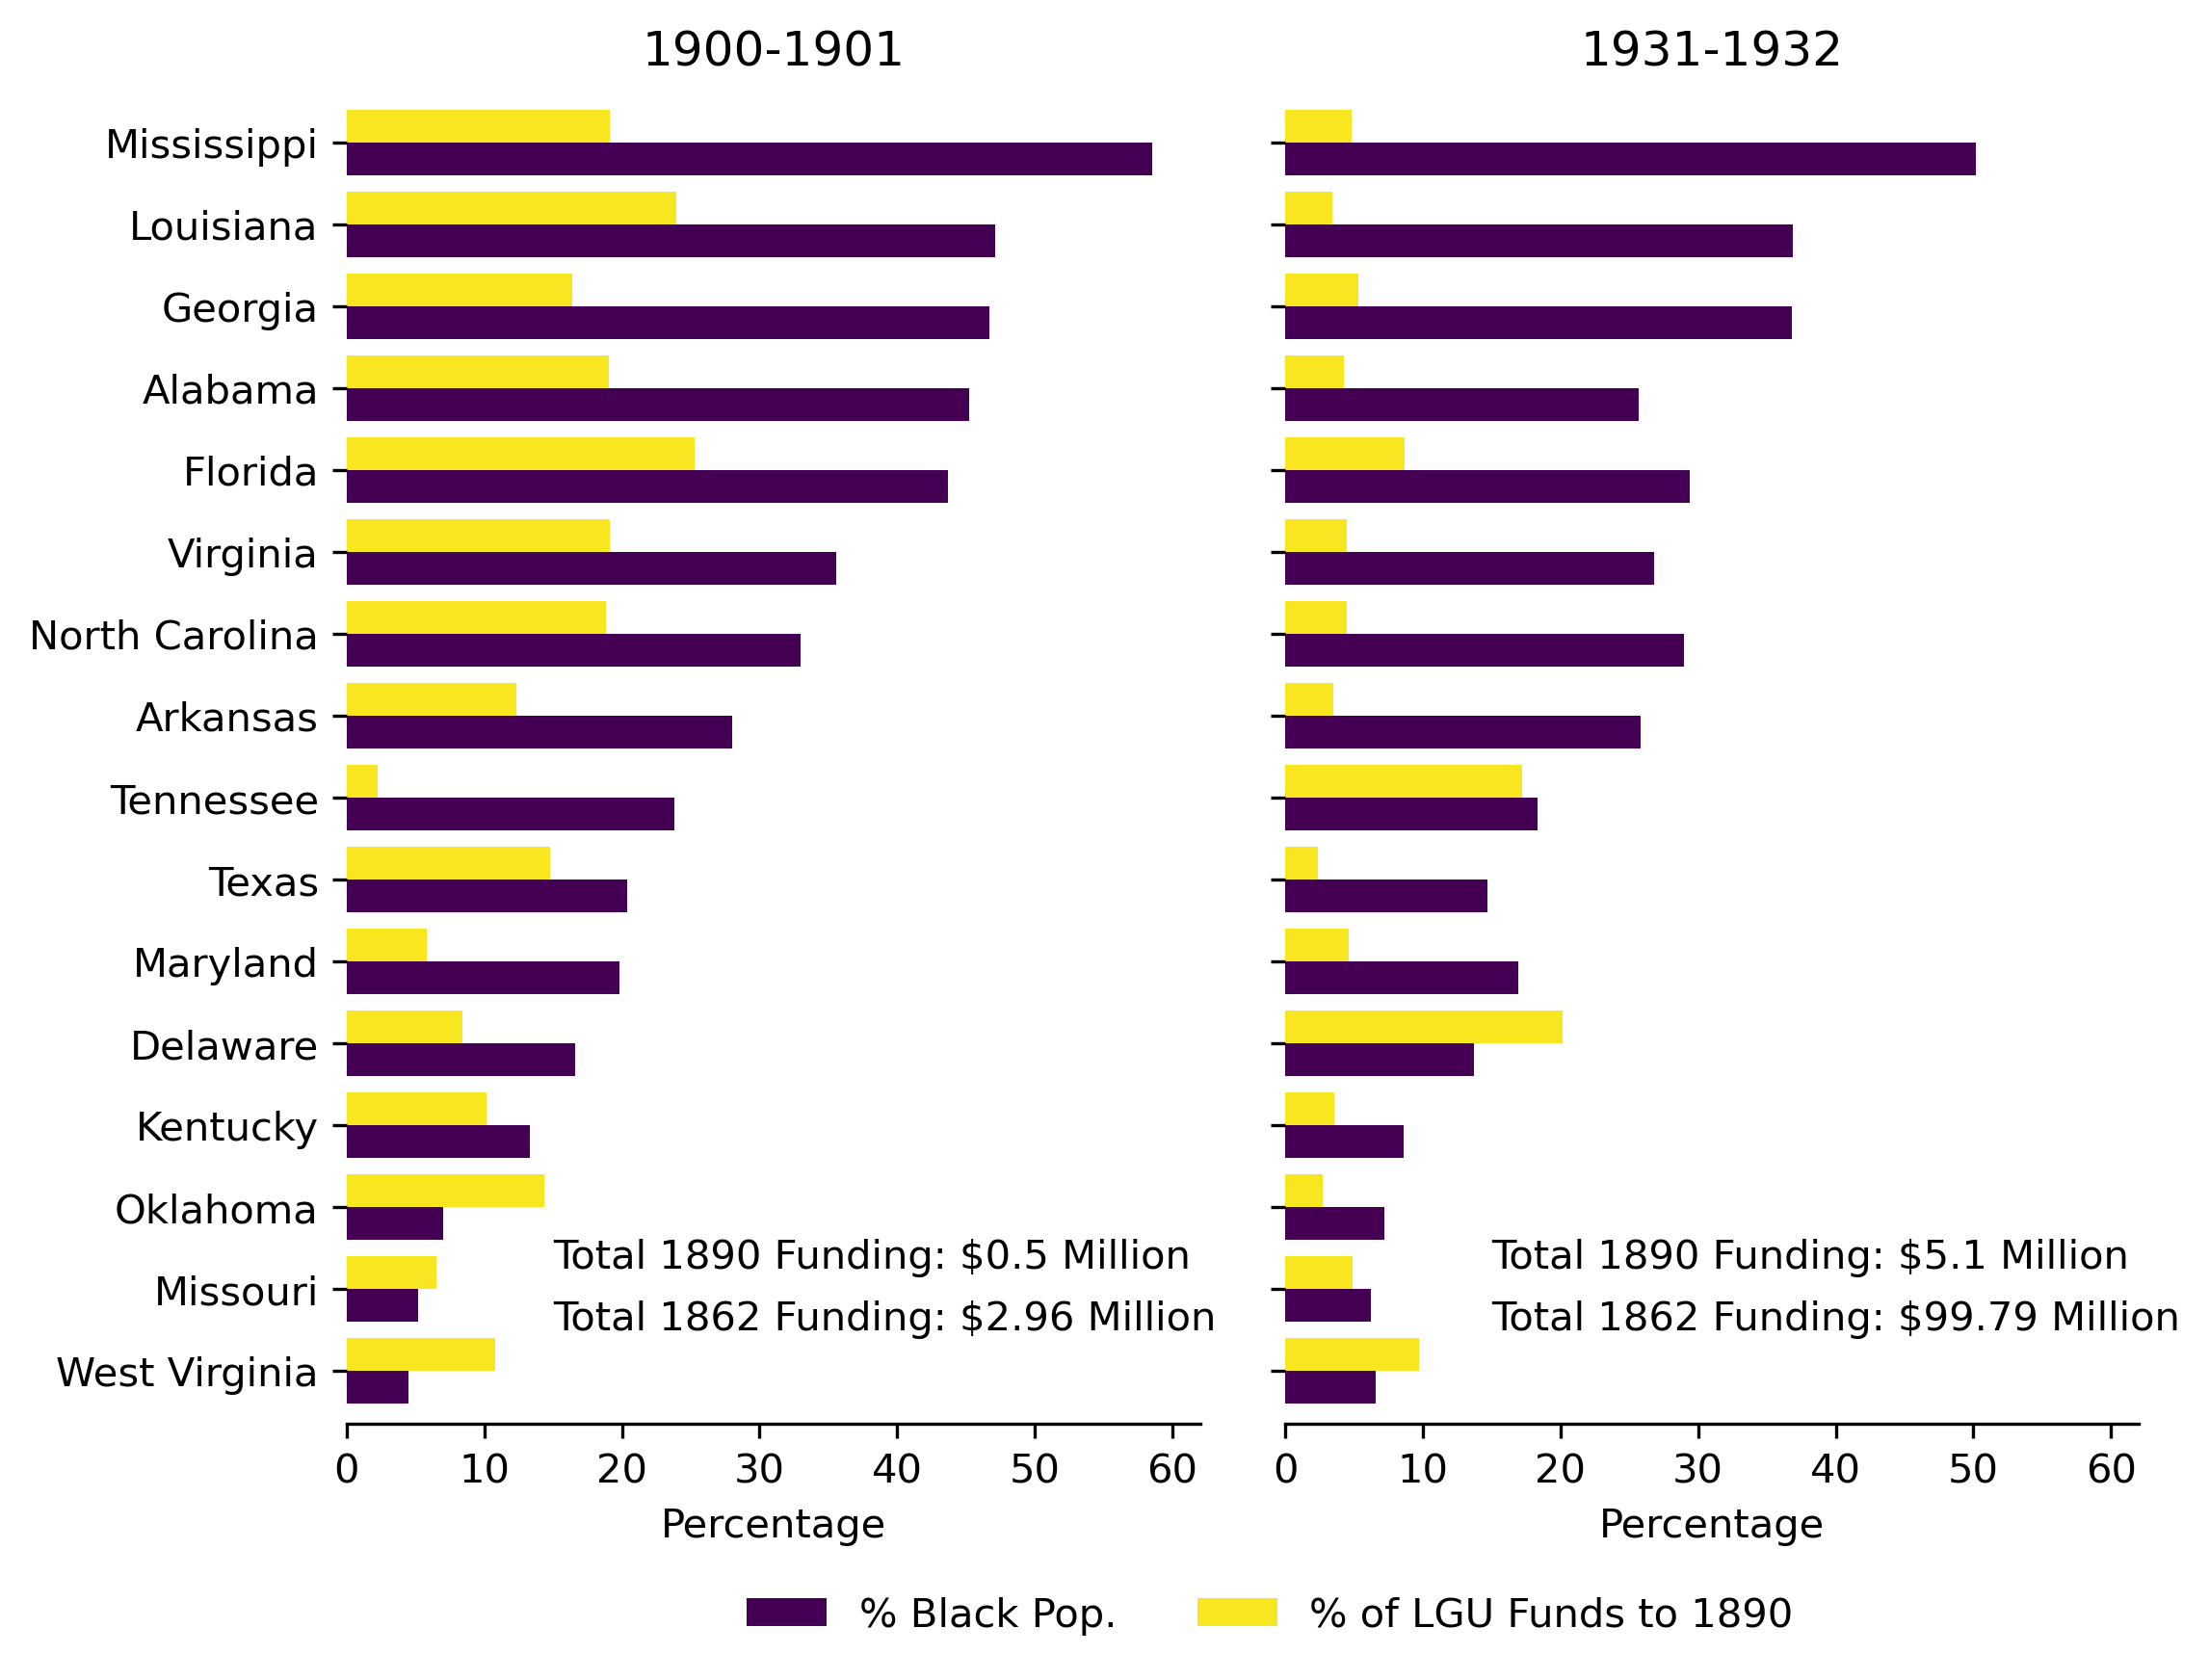
\includegraphics[width=.9\textwidth]{figs/Figure2.png}

Source: Davis (1938), Table 3 pg. 289. 

Note: States are sorted by percentage of population that is Black in 1900.
\end{figure}

Data on funding levels for the 1862 and 1890 LGUs are made available through statistical bulletins published by the Bureau of Education.
When adjusting for the levels of students, 1890 LGUs received about \$100 per student compared to \$265 per student at 1862 LGUs from 1912 to 1913.
The disparity was smaller but largely unchanged in 1923, with 1890 LGUs receiving \$147 per student and \$334 per student at 1862 LGUs \citep{greenleaf_statistics_1926}.\footnote{Author's calculations using tables 1 and 16 of \citet{greenleaf_statistics_1926}, dividing the total income in each year by the number of enrolled students.}
In terms of total funding levels, more comprehensive data from these bulletins are summarized in \citet{davis_participation_1938} for select years from the 1900-1901 school year to the 1931-1932 school year.
Figure \ref{1890LGUfunds} visualizes data from table 3 of the paper which breaks down funding levels by state and compares it to the percentage of the population that is Black in the nearest Census year in 1900-1901 and 1931-1932.

There are at least two important takeaways from these data.
First, the budget for the 1890 LGUs grew modestly in 30 years, from \$0.5 million to \$5.1 million, while the 1862 budget saw a more than 30-fold increase, from \$2.96 million to about \$100 million.
Second, the percent of the funds given to 1890s was not in proportion to the Black population in the majority of states in either year.
On aggregate, the 1890 LGUs were given about 14\% of total funds in 1900 but less than 5\% in 1931.
At the state level, the proportion to 1890s was not in proportion with the Black population in any of the states with more than 30\% of their population being Black, meaning Southern states like Mississippi, Louisiana, and Georgia.
However, some states gave a proportion to the 1890s that was more in line with their population such as Tennessee, Oklahoma, West Virginia, and Delaware.


\begin{figure}
\caption{Funding to 1890 LGUs and Negro Extension Service versus Black Population: 1930, 1932, and 1937}
\label{1890funds_ext}
\centering
    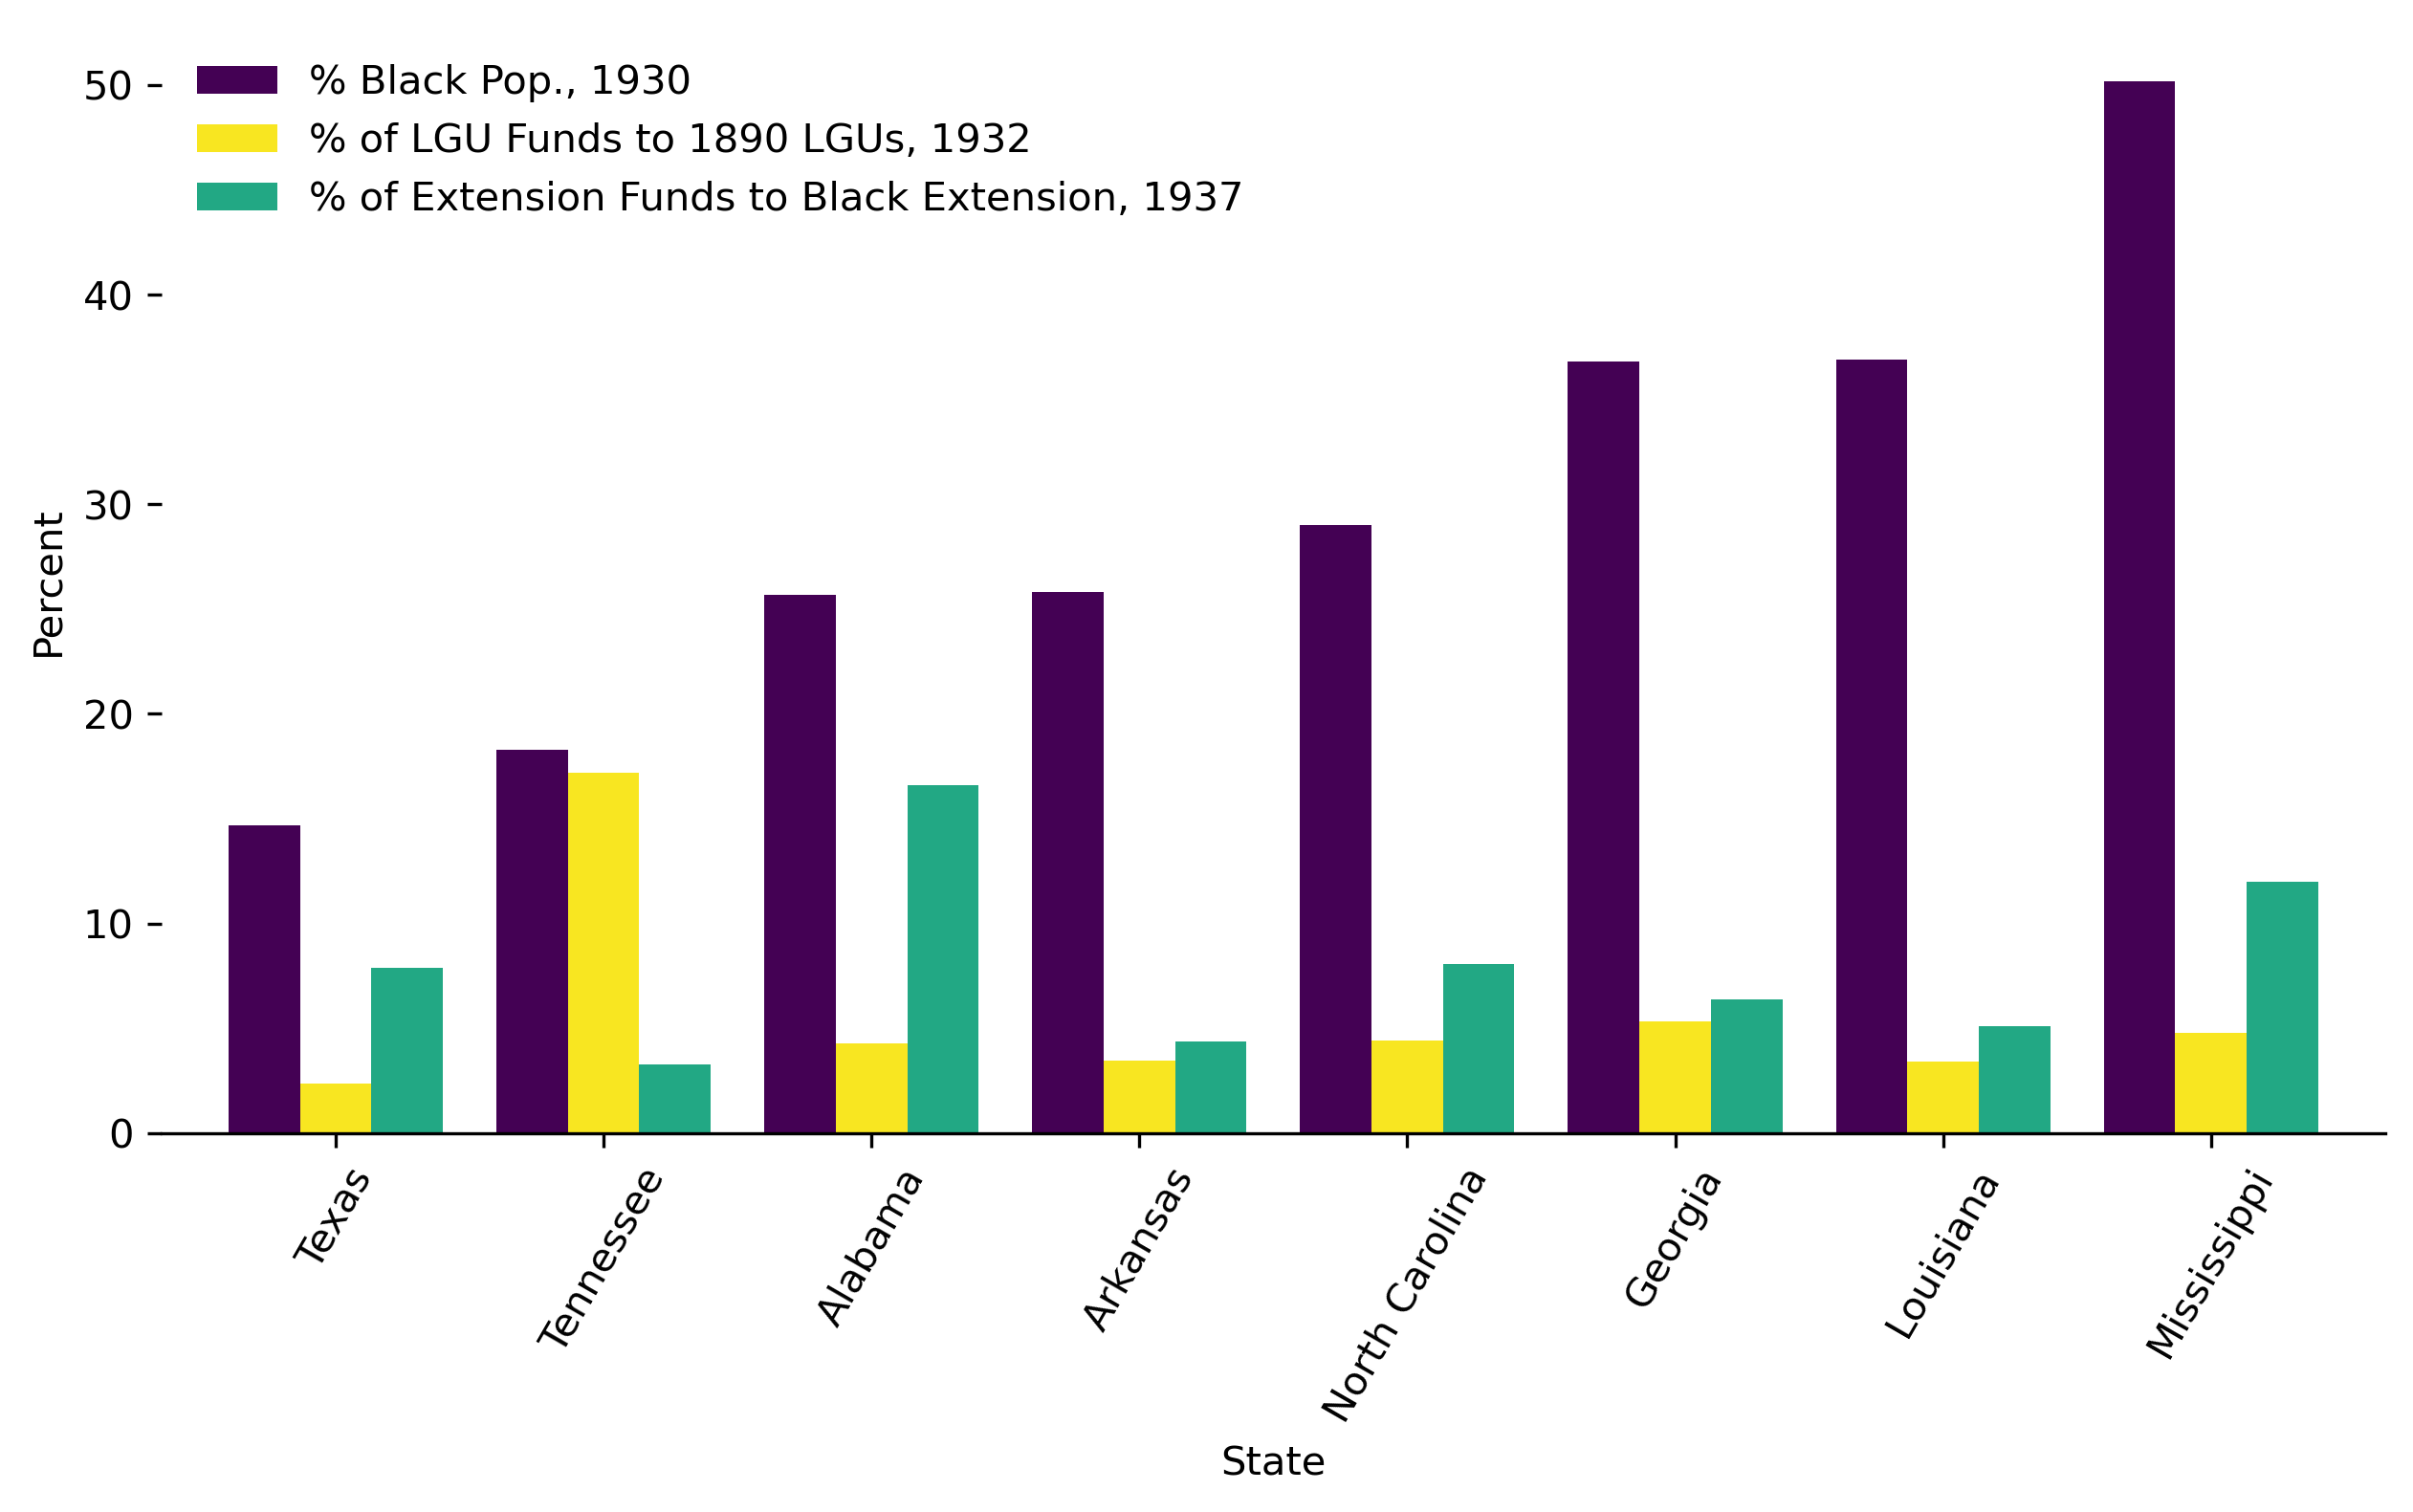
\includegraphics[width=.9\textwidth]{figs/Figure3.png}

Source: Davis (1938), Table 3 pg. 289 and Baker (1939), Table 21 pg. 198 

\end{figure}

\citet{baker_negro_1939} tabulates additional data for 1937 on proportional funding to Black extension programs in selected states.
Figure \ref{1890funds_ext} plots these proportions along with the Black population percentage in 1930 and the proportion of total funds to 1890 LGUs in 1932.
Extension funding in all these states fell short of the Black population percentage in the last available Census; Alabama is the only state that gave its 1890 more than 10\% of the extension funds.
Since LGU funds were intended to be proportioned based on population percentages, this disparity across total funds and extension funds suggested to critics that some state legislatures were not dispersing funds in the spirit of the 1890 Morrill Act, that is in a manner that was ``\textit{just and equitable}'' \citep{davis_participation_1938,wilkerson_agricultural_1942}.
 

Another data source for understanding disparities in the extension program is caseloads for Black and white extension agents. 
Both \citet{wilkerson_agricultural_1942} and the Commission on Civil Rights found that, due to a shortage of agents, caseloads were at least double for Black extension agents. 
In Alabama, there were 796 Black farmers per Black extension agent compared to 312 white farmers per white extension agent in 1964. 
In Mississippi, Black agents had a three-times higher caseload (945 versus 310). The discrepancy was even greater in youth programs where Black extension agents had a four times higher caseload than white extension agents \citep[pg. 43]{us_commission_on_civil_rights_equal_1965}. 

Studies on the economic implications of these funding disparities for Black farmers during this period are rare, if not nonexistent, in economics.
Studies looking at current disparities between 1862 and 1890 LGUs are more common.
For example, \citet{grant_overview_2024} finds that 1890 LGUs today have fewer faculty with lower salaries and less access to state-of-the-art research facilities and technologies compared to their 1862 counterparts. \citet{wilson_distribution_2024} analyzes grant funding patterns for 1890 LGUs and similarly finds that a lack of resources has also led to less success in grant activity. 
\citet{wilson_distribution_2024} attributes this competitive funding disparity to factors including lower financial and research capacity and human capital at 1890 LGUs due to a relative lack of initial endowments.

\section*{Financial Assistance Policy}
A final, critical factor in the technological treadmill is government financial assistance in the form of loans and subsidies.
Starting with the Agricultural Adjustment Act (AAA) of 1933, for the next thirty years the USDA paid farmers to control their acreage by either plowing under existing production or setting aside land from production. 
Government payments became an important respite for farmers from dropping commodity prices after World War II and productivity growth that continued to expand production.
In the technological treadmill, subsides are key for not only softening the blow of these price drops but also loosening credit constraints to increase technology adoption.

An important feature of the new policy apparatus was that benefits were primarily controlled by local, county committees. 
Committee members were elected democratically by the local farmers in the community and were in charge of screening applicants for payments. 
This practice continued with practically every subsidy or loan program, including the Bankhead-Jones Farm Tenant Act of 1937 \citep[pg. 478]{banfield_ten_1949}, the Farmer’s Home Administration loan program \citep[pg. 61]{us_commission_on_civil_rights_equal_1965}, and the Agricultural Stabilization and Conservation Service (formerly known as the Agricultural Adjustment Administration). 
County committees also had an extraordinary amount of influence in determining the amount of land a farmer was allowed to set aside, the size of the benefits, and whether appeals would be heard or not \citep{us_commission_on_civil_rights_equal_1965}. 

Black farmers had minimal participation on these committees, a fact which greatly reduced their access to financial support \citep{jones_negro_1953}.
The Civil Rights Commission report found that, in 1964, only 75 out of 37,000 committee members in the South (about 0.2\%) were Black. 
Similarly, there were no Black committee members on any of the committees in charge of FHA loans in 1961 \citep[pg. 60]{us_commission_on_civil_rights_equal_1965}. 
In thirty years of federal policy, not one Black farmer had been appointed to a state-level committee by the Secretary of Agriculture. 
This is despite the fact that 92\% of Black farmers in the South were growing program-eligible crops like cotton, tobacco, and peanuts \citep[pg. 90-91]{us_commission_on_civil_rights_equal_1965}. 
Moreover, Black farmers reported that they did not have recourse to complain about the lack of representation for fear of retaliation by officials \citep{baker_negro_1939}. 

Attempts to increase the representation of Black farmers on the committees were often met with significant opposition in the Southern states. 
When Civil Rights activists working with the Council on Federated Organizations attempted to increase the representation of Black farmers on county committees in the Southern states, local white farmers and local officials often rallied together to keep Black farmers from being elected. 
The Mississippi State Sovereignty Commission, formed in 1956 to resist integration, aimed in 1964 to increase white turnout in the county committee elections to counter increases in Black farmer voting \citep{irons_reconstituting_2010}. 
This happened in parallel to the USDA denying ballots to Black tenants and sharecroppers and ignoring reports of Black farmers being physically threatened at polling locations in county committee elections  \citep{daniel_dispossession_2013}. 

The high rates of tenancy among Black farmers put them at an additional disadvantage in the programs since tenants were absent from county committees and had to receive their share of payments from the landowners.
In the case of cotton, only landlords were allowed to sign production control contracts and receive payments since tenants and sharecroppers had no “legal claim” on the crop \citep[pg. 52]{conrad_forgotten_1965}. 
Landlords were at least on paper required to distribute their payments to their tenants, a provision that USDA officials internally admitted was not legally enforceable \citep[pg. 58]{conrad_forgotten_1965}. 
%When asked why tenants were not on county committees, one county extension agent responded, “you wouldn’t put a chicken on a poultry board, would you?” \citep[pg. 81]{conrad_forgotten_1965}. 

Since production control contracts required farmers to take land out of production, landowners even opted to evict tenants and fire sharecroppers when given subsidies. 
In Alabama, a survey found that about half of landlords stated that they had evicted tenants due to reduced acreage or uncertainty around payments for acreage reduction.
The same survey found that 40\% of landlords opposed granting relief to tenants specifically for fear that it would improve the bargaining position of their tenants \citep{conrad_forgotten_1965}. 

\begin{figure}[ht!]
    \centering
    \caption{FHA Loans per \$1,000 of Net Worth by Race and Economic Class}
    \label{fhaloans}
    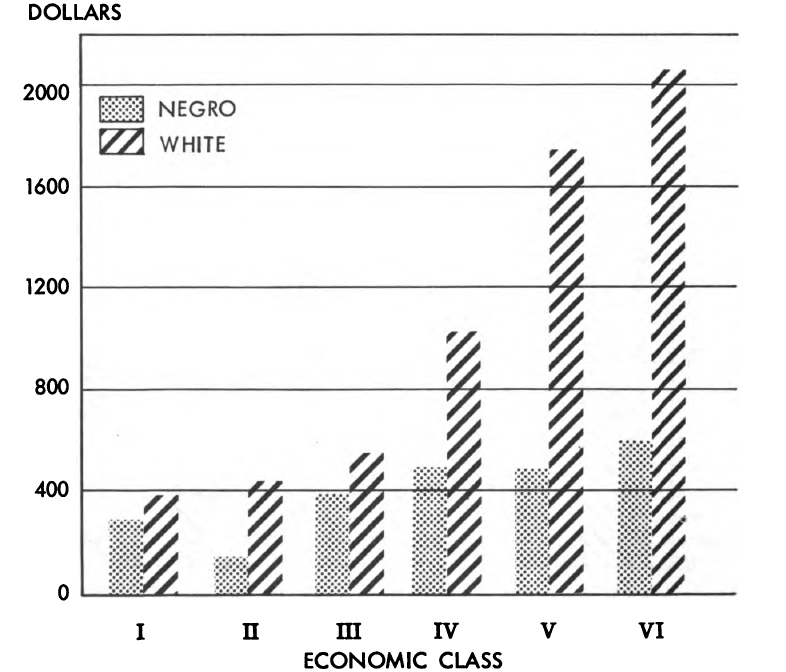
\includegraphics[width=.75\textwidth]{figs/Figure4.png}
   \begin{minipage}{.8\textwidth}
    \centering
    \quad \\
    Source: \citet{us_commission_on_civil_rights_equal_1965}, Figure 2 pg. 70. 
    \quad \\
    \quad \\
    ``Economic Class'' refers to categories of net worth where Class I is over 20 thousand dollars, Class II between 15 and 20 thousand, Class III between 10 and 15 thousand, Class IV between 6 and 10 thousand, Class V between 3 and 6 thousand, and Class VI less than 3 thousand
    \end{minipage}
\end{figure}

 The Civil Rights Commission provides one of the earliest analyses of racial disparities in loan programs. 
 Specifically, they studied loan data from the FHA program from 1963 to 1964 and found that Black applicants with the same amount of net worth received much smaller loans than their white counterparts \citep[pg. 71]{us_commission_on_civil_rights_equal_1965}. 
 Figure \ref{fhaloans} shows the average loan size per dollar of net worth for Black and white borrowers across “economic class,” where class I is the highest income and class VI is the lowest. 
 Comparing Black and white borrowers by this metric, amount of loan per thousands of dollars of net worth, is intended to adjust for the fact that higher net worth individuals receive larger loans. 
 This graph indicates that Black borrowers across all wealth categories benefited less than their white counterparts: the poorest Black applicants received only \$500 for each additional \$1,000 in net worth versus \$2,000 for the poorest white borrowers. 

While payments and loans today are far less subject to the whims of the county committees, many studies continue to find disparities in subsidy and loan programs.
Analyses of more recent Farm Service Agency loan data continue to find racial and gender disparities in lending \citep{escalante_credit_2006,ghimire_farm_2020,mishra_racial_2024,vekemans_loan_2024}. 
Racial disparities in access to government payments have also been noted in ad-hoc payments: the Market Facilitation Program (MFP) and the Coronavirus Food Assistance Program (CFAP) \citep{giri_analysis_2022,hendricks_explaining_2024,yu_understanding_2024}.
A common finding from these studies is that some of these disparities can be partly explained by the fact that Black farmers today usually have smaller farms and fewer assets.

\section*{Discussion and Future Research Directions}
Understanding how racial discrimination has mediated structural change impacts on Black farmers is crucial for understanding the current policy debate around racial inequity in agriculture.
Efforts to address disparities have been most successful in financial assistance and education, while reversing land losses has proved less successful. 
Yet, all of these policy efforts have emerged from a historical context that the field of agricultural economics has analyzed very little.
To conclude this paper, we discuss some of the current policy environment in these three areas and offer future directions for research in racial inequity in US agriculture.

While the bulk of the reduction in Black farmers happened before 1970, the class action lawsuit Pigford v Glickman uncovered numerous instances of racial discrimination in loans and disaster assistance between 1983 and 1997. 
By 2012, at least \$1 billion in settlements had been paid to claimants by the USDA, making it the biggest class action lawsuit against the US government in US history \citep{cowan_pigford_2013}. 
Apart from the Pigford settlements, the US government has taken additional policy measures intending to prevent future discrimination.
The Agricultural Credit Act of 1987 also set annual target participation rates for minority farm operators at the county level to ensure equitable lending (P.L. 100-233; 7 U.S.C. §2003). 
The Department of Agriculture Reauthorization Act of 1994 also significantly reduced the power of county committees to make unilateral decisions about loans and subsidies, instead giving that authority to Farm Service Agency personnel (P.L. 103- 354). 
This lessened the ability of county committees to discriminate based on race by providing a degree of federal oversight to decisions about loans and subsidies. 

The most recent policy efforts to address racial discrimination in financial assistance have addressed a much broader category of farmers: socially-disadvantaged farmers and ranchers (SDFRs).
In 2021, Senator Raphael Warnock introduced the Emergency Relief for Farmers of Color Act which allocated \$5 billion to debt relief (\$4 billion), technical training, and funding for the 1890 LGUs (\$1 billion) \citep{warncock_relief_2023}. 
This became Section 1005 of the American Rescue Plan Act (ARPA), a COVID relief bill passed in 2021. 
Section 1005 also created an Equity Commission within the USDA to investigate racial discrimination in USDA programming \citep{yarmuth_american_2021}. 
Several lawsuits from white farmers alleging racial discrimination stopped the ARPA debt relief from going out. 
The Inflation Reduction Act of 2022 repealed Section 1005 and instead provided debt relief for “economically distressed farmers,” a category that was broader still and included some white farmers \citep{bustillo_black_2023}. 

In the area of education, it took more than eighty years for the 1890 schools to receive their own research and extension funding. 
The 1890 LGUs finally received dedicated funding for research through the Evans Allen Act of 1977 and for extension through the National Agricultural Research, Extension and Teaching Policy Act of 1997 \citep{tegene_investing_2002}. 
However, all LGUs are required to match 100\% of federal funds with other funds (usually the state legislature) or 50\% if the USDA grants them a waiver. 
Many 1890 LGUs have not been able to match even 50\%, meaning they have had to forfeit their federal funding. 
From 2010 to 2012, 1890 LGUs had to forfeit \$31 million in federal funding due to failure to match \citep{lee_land-grant_2013}. 
Another analysis estimates that state legislatures have denied 1890 LGUs a total of \$12 billion in funding originally allocated for them by failing to match between 1987 and 2020 \citep{adams_how_2022}. 

Addressing land loss with policy has proved more challenging.
One of the earliest efforts was led by the economist Robert S Browne, who established the Black Economics Research Center (BERC) in 1969 and the Emergency Land Fund (ELF) in 1971 to raise money to help Black farmers buy back their land lost through foreclosure \citep{handy_emergence_2008}. 
Black farmer organizations such as The Colored Farmers National Alliance and Cooperative Union, established in 1886, also helped address the discrimination facing Black farmers by purchasing land for Black farmers and providing loans \citep{white_freedom_2019}. 
The Justice for Black Farmers Act (JBFA), introduced in 2021 and 2023 but never passed, appeared to be the modern manifestation of these efforts.
The most ambitious part of the bill was a plan to allocate \$8 billion to the USDA to buy farmland from “willing sellers” and transfer it to Black farmers \citep{booker_justice_2023}. 
The JBFA aimed to also address disparities in education and financial assistance by allocating \$500 million each year to the 1890 LGUs and using \$1 billion to establish a “National Socially Disadvantaged Farmer and Rancher Bank” which will make loans to credit institutions where at least 60\% of their members are socially disadvantaged farmers \citep{booker_justice_2023}.

Yet, it does not appear that any of these policies have had significant impacts on the number of Black farmers: in 2022, there were even fewer Black farmers, 1.4\% of operators, than in 1969, 3.2\% of operators \citep{USDA_black_farmers}. 
To understand how policy might impact Black farmers, future research can start by understanding the policy dynamics of 1920-1970, the period in which the number of Black farmers declined the strongest. 
In this paper, we describe several areas of policy that have appeared to influence the outcomes of the technological treadmill yet are not as investigated in the field of economics.
In particular, there are several future research directions that may be fruitful avenues for better understanding racial discrimination and structural change in US agriculture.

One direction for future research is the role of institutions and political economy in the disbursement of federal funds in the LGU system and county committees.
Much of the disparities in funding to 1890 LGUs and the Negro Extension Service appear to have been caused by state legislatures exercising significant influence in the distribution of funds.
Similarly, the design of local committee elections seems to have had a large impact on the distribution of payments.
How did political dynamics at the state and local level impact the distribution of extension funding and financial assistance across race?
How have grassroots efforts by discriminated groups countered the impacts of discriminatory policies \citep{smith_ii_food_2023,white_freedom_2019}? 
Finally, what implications did these systems and dynamics have for the success of Black farmers during structural change?
Work in this area requires a firm understanding of the role of institutions in the US agricultural economy that the field of agricultural economics can provide.

Another area for research is specifically understanding the impact of the federal and state underfunding of 1890 LGUs. 
This may be a research gap precisely because the underrepresentation of Black economists in agricultural economics affects the types of topics the field at large decides to study \citep{wilson_call_2023}. 
What political factors determined how resources were distributed at the county level? 
How did the funding gap in extension impact the technology adoption decisions of Black farmers?
Even more importantly, how might initial inequities in LGU and extensions funding in the earliest days of the 1890s perpetuate the inequalities we see today \citep{grant_overview_2024,wilson_distribution_2024}?
More research in this area would be able to provide quantitative evidence for what are currently only case studies from sources such as \citet{us_commission_on_civil_rights_equal_1965} and \citet{black_economic_research_center_center_only_1973}.

Finally, examining racial inequity in US agriculture need not be limited to the Black farmer experience. 
The laggards of Cochrane's treadmill are often those farmers that the federal government has explicitly discriminated against in providing land, education, and financial assistance. 
In this regard, the Black experience in agriculture is not unique. 
Japanese farmers in California were similarly dispossessed of their land by Alien Land Laws in the early 20th century and internment during WWII \citep{arellano-bover_displacement_2022,aoki_no_1998}. 
In addition to the Pigford v Glickman lawsuit, three other lawsuits against the USDA uncovered discrimination against women farmers, Hispanic farmers, and Native American farmers in the USDA loan and subsidy programs \citep{casey_racial_2021}. 
For these farmers, the effects of structural change have likely also been mediated by discrimination.
There is a role for agricultural economics research to similarly provide evidence of the economic impacts of policy on these groups. 


\bibliographystyle{chicago}
\begin{spacing}{1}
\bibliography{bibliography}

\end{spacing}

\newpage
\begin{appendix}
\section*{Online Appendix A: Acreage and Operator Trends, South and Non-South}

One factor that is often mentioned to explain Black farmer decreases is the disproportionate effect that mechanization had on cotton, a crop that many Black farmers grew. While the 1959 Agricultural Census does not break down crops grown by race, it does break down acres and operators by the South and the US as a whole. The 1959 Agricultural Census defines “the South” as 16 states: Delaware, Maryland, Virginia, West Virginia, North Carolina, South Carolina, Georgia, Florida, Kentucky, Tennessee, Alabama, Mississippi, Arkansas, Louisiana, Oklahoma, and Texas. Since the Census measures non-white operators and acreage by tenure status for the South and the whole country, we obtain numbers for “Non-South” by taking the difference between these two totals for 1920 and 1959. This allows us to see whether non-white farmers fared differently outside the South, here a rough proxy for growing certain crops like cotton. 


\begin{table}
\caption{Operators and Acreage by Race, Non-South versus South}
\label{operator_acrage_region}
\centering
\footnotesize
\begin{tabular}{llrrrrrr}
\hline
       &           & \multicolumn{3}{c}{\textit{Non-South}} & \multicolumn{3}{c}{\textit{South}} \\
\multicolumn{2}{l}{Operators (thousands)}&     1920 &     1959 &  \textit{\% Change} &     1920 &    1959 &  \textit{\% Change}\\
[.5em]
\hline
Owner & White &  1,947.47 &  1,159.94    &    \textit{-40.44} &  1,227.20 &  856.86 &    \textit{-30.18} \\
       & Non-white &    14.57 &     7.64 &    \textit{-47.56} &   178.56 &   89.75 &     \textit{-49.74} \\
       [1em]
Part Owner & White &   365.39 &   507.00 &     \textit{38.76} &   152.43 &  285.42 &    \textit{ 87.24} \\
       & Non-white &     1.86 &     3.20 &     \textit{72.27} &    39.03 &   37.53 &    \textit{ -3.84} \\
       [1em]
Tenant & White     &   852.97 &   364.20 &    \textit{-57.30} &   887.57 &  228.22 &    \textit{-74.29} \\
       & Non-white &    14.45 &     2.97 &    \textit{-79.46} &   703.56 &  138.05 &    \textit{-80.38} \\
       [.5em]
\hline \hline 
       &           & \multicolumn{3}{c}{\textit{Non-South}} & \multicolumn{3}{c}{\textit{South}} \\
       % &           &     1920 &     1959 &  \% Change &     1920 &     1959 &  \% Change \\
\multicolumn{2}{l}{Acres (millions)} &     1920 &     1959 &  \textit{\% Change} &     1920 &    1959 &  \textit{\% Change}\\
[.5em]
\hline
Owner & White      &  2,775.42 &  2,014.20 &    \textit{-27.43} &  1,697.03 &  1,383.98 &    \textit{-18.45} \\
       & Non-white &    20.55  &    10.07  &    \textit{-50.99} &   119.50 &    55.77 &      \textit{-53.33} \\
       [1em]
Part Owner & White &  1,360.04 &  3,636.42 &    \textit{167.38} &   368.22 &  1,339.57 &    \textit{263.80} \\
       & Non-white &     5.73  &    22.29  &    \textit{289.27} &    21.26 &    31.04  &    \textit{ 45.97} \\
       [1em]
Tenant & White     &  1,570.10 &  1,119.32 &    \textit{-28.71} &   802.05 &   457.09 &    \textit{-43.01} \\
       & Non-white &     8.91  &     6.74  &    \textit{-24.35} &   268.74 &    48.69 &    \textit{-81.88} \\
       [.5em]
\hline \hline 
\end{tabular}
\normalsize

Source: US Agricultural Census 1959, Chapter X, Tables 4-7
\end{table}


Table \ref{operator_acrage_region} shows the same numbers as table \ref{operator_acrage} but broken down by South and Non-South. While there are fewer non-white farmers outside of the South, there are similar disparities across race both in and outside of the South. Non-white owners in either region lost about the same percentage of operators, 47-49\%, while white owners decreased between 30 and 40\%. While the South lost roughly the same percentage of tenants regardless of race, outside the South there were larger decreases in non-white tenants (-79\%) than white tenants (-57\%). Much like the rest of the country, the biggest disparities across race in either region were in acreage: non-white owners in either region lost about half of their acreage while white owners only lost at most 27\% of their acreage. While cotton mechanization is one factor in Black farmer exit, large racial disparities in losses outside the South suggest it does not fully explain the decrease in those forty years.

\end{appendix}

\end{document}
